\documentclass[11pt,a4paper]{article}
\usepackage[top=21mm,bottom=22mm,left=23mm,right=23mm,headheight=15pt]{geometry}
\usepackage{fontspec,amsmath,amssymb,mathtools,booktabs,longtable,tabularx,array,graphicx}
\usepackage{xcolor,enumitem,fancyhdr,titlesec}
\usepackage[hyphens]{url}
\usepackage{xurl}
\usepackage[colorlinks=true,linkcolor=blue!45!black,urlcolor=blue!45!black]{hyperref}
\setmainfont{TeX Gyre Pagella}
\setmonofont[Scale=0.80]{DejaVu Sans Mono}
\hypersetup{pdftitle={Chapter 3: Independent Manuscript Audit},pdfauthor={Archon Horizon / ArakelovGeometry},pdfsubject={Chen--Moriwaki v1.2 and formalization fe4feea}}
\definecolor{navy}{HTML}{173D58}
\titleformat{\section}{\Large\bfseries\color{navy}}{\thesection}{0.6em}{}
\titleformat{\subsection}{\large\bfseries\color{navy}}{\thesubsection}{0.6em}{}
\pagestyle{fancy}\fancyhf{}
\fancyhead[L]{\small Chapter 3: Independent Manuscript Audit}
\fancyhead[R]{\small Chen--Moriwaki v1.2}
\fancyfoot[L]{\footnotesize 2026-10-02\quad ·\quad ArakelovGeometry}
\fancyfoot[R]{\small\thepage}
\setlength{\parskip}{4pt}
\setlength{\emergencystretch}{3em}
\setlist{nosep,leftmargin=1.8em,topsep=4pt}
\newcommand{\Q}{\mathbb Q}
\newcommand{\R}{\mathbb R}
\newcommand{\C}{\mathbb C}
\newcommand{\Z}{\mathbb Z}
\newcommand{\A}{\mathcal A}
\newcommand{\E}{\mathcal E}
\newcommand{\PP}{\mathbb P}
\newcommand{\code}[1]{{\small\nolinkurl{#1}}}
\newcommand{\loc}[2]{\par\noindent\textbf{Source:} PDF pp.~#1; printed pp.~#2.}
\newcommand{\verdict}[1]{\par\noindent\textbf{Verdict:} #1\par}
\newcolumntype{Y}{>{\raggedright\arraybackslash}X}
\begin{document}
\thispagestyle{plain}
\begin{center}
{\LARGE\bfseries\color{navy}Chapter 3: Independent Manuscript Audit}\\[7pt]
{\large Huayi Chen and Atsushi Moriwaki}\\[3pt]
{\itshape Arakelov geometry over adelic curves}\\[4pt]
{Version 1.2, 5 October 2019}\quad\textbar\quad{Audit: 2 October 2026}
\end{center}

This retrospective review separates manuscript defects, notation slips, earlier review overclaims, and formalization boundaries. Three substantive findings survive independent scrutiny: \textbf{a false degree-divisibility step in the algebraic tower proof; a false identification of the cylinder and full Borel $\sigma$-algebras; and an error term that need not be finite in the Northcott proof.} Each admits a repair preserving the intended main theorem.

\begin{center}\small
\begin{tabularx}{\linewidth}{@{}lYl@{}}\toprule
Priority / ID & Finding and classification & Report page\\\midrule
High S1 & False divisibility; substantive proof error & \pageref{s1}\\
High S2 & False Borel equality inside the probability proof & \pageref{s2}\\
High S3 & Infinite mass cannot supply a finite Northcott bound & \pageref{s3}\\
Medium T13 & Horizontal infinity mistakenly included in a recalled definition & \pageref{horizontal}\\
Low (other T) & Notation/reference corrections; T6 partly withdrawn & \pageref{notation}\\
Notes E1--E3 & Expository qualifications, not additional major errors & \pageref{e1}\\
Boundary F1--F3 & Formalization corrections and a normalization difference & \pageref{formal}\\\bottomrule
\end{tabularx}
\end{center}

\noindent\textbf{Pinned objects.}
Reviewed Horizon ledger revision:
\code{fe4feea1cf1c818fc0011473b31e9205687c6f66}.
The original PDF has 466 pages; its cover visually confirms the version and date.
Its SHA-256 is
\begin{quote}\small\ttfamily
83ccb69c22ad7d449248bbb26c48216d9b41\\
4f672af6f7f4f172d5ba17be57cc
\end{quote}
PDF locators are \emph{one-based viewer pages}. In the cited body, PDF page equals printed page plus 16. These locators are version-specific.

\noindent\textbf{Method and limits.}
Claimed defects were checked against rendered original pages and their hypotheses, then against the source-result index, blueprint, Lean statements, and relevant proof bodies. Three focused reviewers and a separate mathematical adjudicator supplied independent checks. The older report was treated as a list of hypotheses. Accepted Lean, blueprint, configuration, and old reports were left unchanged. This is not an audit of the entire book or a fresh Lean certification. Appendices give coverage and exact code locations; \code{findings.json} is the evidence catalogue.

\clearpage
\section{S1: false degree divisibility in finite descent}\label{s1}
\loc{212--214}{196--198}
Theorem 3.4.12 is stated on PDF p.~212. The defect occurs on p.~213, after the first tower-integral display, in the paragraph beginning “Otherwise one has”. With $K_1=K_2\cap L_1$, the manuscript asserts
\[
 [K_2:K_1]\mid[L_2:L_1],\qquad
 [K_2:K_1]=[L_2:L_1]\quad\text{when the latter is prime}.
\]
\verdict{Confirmed manuscript proof error; high confidence. The counterexample satisfies the relevant hypotheses preceding this assertion.}

Let $a=\sqrt[3]{2}\in\R$, let $\zeta$ be a primitive cube root of unity, and set
\[
 K=\Q,\qquad K_2=\Q(a),\qquad L_1=\Q(\zeta a),\qquad L_2=\Q(a,\zeta).
\]
Eisenstein's criterion makes $T^3-2$ irreducible, so both cubic subfields have degree 3. They are distinct: $K_2$ is real whereas $\zeta a\in L_1$ is not. Their intersection has degree dividing 3; degree 3 would force equality, so $K_1=\Q$. Since $\zeta$ is quadratic over the real field $\Q(a)$, $[L_2:\Q]=6$. Moreover, $a$ and $\zeta a$ generate $L_2$. Consequently
\[
 [K_2:K_1]=3,\qquad [L_2:L_1]=2,\qquad 3\nmid2.
\]
The source assumes successive algebraic extensions $L_2/L_1/K$. Here all extensions are finite and separable, $K_2/K$ is finite, $K_2\not\subset L_1$, and the upper degree is prime. There is no relative algebraic-closure assumption excluding this example. The usual adelic curve on $\Q$ supplies valid base-curve data; this is a counterexample within the source hypotheses, not merely to an unrelated field-theoretic statement.

\subsection{Two qualifications to the older report}
The preceding “By induction it suffices” reduction to prime upper degree also needs justification: an arbitrary finite extension does not automatically admit a tower whose successive degrees are prime. The displayed counterexample already defeats the core step even if the prime-degree reduction is granted.

The older report separately objects that the chosen polynomial $P$ need not remain minimal over $L_1$. That objection needs qualification. If one grants the manuscript's preceding assertions
\[
 [K_2:K_1]=[L_2:L_1]=p,\quad K_2=K_1(a),\quad L_2=L_1(a),
\]
then the minimal polynomial over $L_1$ divides $P$ and both have degree $p$. Thus $P$ does remain minimal under those asserted equalities. The cubic example refutes the upstream degree assertion; it is not another counterexample satisfying that assertion. The later factor and weight computations inherit the failure of the degree setup.

\subsection{Repair and effect on the theorem}
Finite descent must allow a sufficiently large finite base field, instead of forcing the base to be the intersection with an arbitrarily chosen finite field. For algebraic $B/K$, finite $N/B$, and a finite intermediate $F/K\subset N$, descend a basis, its multiplication constants, the needed elements of $F$, and the separable part. This yields finite $A/K\subset B$ and finite $E/K\subset N$ with
\[
 A,F\subset E,\qquad BE=N,\qquad
 [E:A]=[N:B],\qquad [E:A]_{\rm s}=[N:B]_{\rm s}.
\]
Base change and embedding counts then give compatible local probability weights. Prove the tower identity on finite cylinders and extend by uniqueness of finite measures on a generating $\pi$-system. This repairs the proof of Theorem 3.4.12 without refuting its conclusion.

The repair uses \code{IntermediateField.exists_finite_descent}; Appendix A identifies its cylinder and measure consumers and exact blueprint attachments.

\clearpage
\section{S2: cylinder measurability need not equal full Borel measurability}\label{s2}
\loc{208--209}{192--193}
The penultimate main paragraph on PDF p.~208 defines $\A_{L,\omega}$ as the smallest $\sigma$-algebra making all restrictions to finite stages measurable. The proof of Proposition 3.4.6 on p.~209 calls it “the Borel algebra of the projective limit topology” and again calls the resulting probability Borel at the end.
\verdict{Confirmed false assertion inside the proof; high confidence. An actual adelic fibre furnishes a counterexample. The stated cylinder-probability existence conclusion survives.}

For uncountable $I$, every set in the cylinder $\sigma$-algebra of $\{\pm1\}^I$ depends on at most countably many coordinates: the class of such sets contains finite cylinders and is closed under complements and countable unions. A singleton is closed in the product topology and hence Borel, but it cannot depend on only countably many coordinates.

That observation alone refutes only a \emph{general} inverse-limit inference. The following construction verifies that the same failure occurs within the manuscript's precise adelic setting.

\subsection{An uncountable multiquadratic fibre}
Choose algebraically independent $y_i$ for an uncountable index set $I$, and put
\[
 L=\Q(y_i:i\in I),\qquad x_i=y_i^2-1,\qquad K=\Q(x_i:i\in I).
\]
The $x_i$ are algebraically independent: substitution $X_i\mapsto Y_i^2-1$ is injective on every finite polynomial ring. Each $y_i$ satisfies $y_i^2=1+x_i$, so $L/K$ is algebraic.

On nonzero rational functions in the $x_i$, define
\[
 v(P/Q)=\operatorname{ord}_0(P)-\operatorname{ord}_0(Q),\qquad |f|=2^{-v(f)},
\]
where $\operatorname{ord}_0$ is the lowest nonzero \emph{total degree}. Every polynomial uses finitely many variables, and products of lowest homogeneous forms remain nonzero. Thus this is a well-defined discrete valuation. It is trivial on $\Q^\times$, and $|x_i|=1/2$. No assertion that its residue field is $\Q$ is needed.

Use a one-point parameter space of mass 1 carrying this absolute value. Every nonzero logarithmic evaluation is a finite constant, hence measurable and integrable. This satisfies the adelic-curve definition in \S3.1. The curve is not proper, but \S3.4 and Proposition 3.4.6 require neither properness nor countability of the field. Countability on PDF p.~185 is a hypothesis of Proposition 3.1.3 only.

For $\varepsilon\in\{\pm1\}^I$, take the total-degree valuation $w_\varepsilon$ at $y_i=\varepsilon_i$. With $z_i=y_i-\varepsilon_i$,
\[
 x_i=2\varepsilon_i z_i+z_i^2.
\]
Substitution preserves each lowest nonzero homogeneous degree, so $w_\varepsilon|_K=v$. These extensions are distinct, since
\[
 |y_i-1|_\varepsilon=
 \begin{cases}1/2,&\varepsilon_i=1,\\1,&\varepsilon_i=-1.\end{cases}
\]

\subsection{Why these are all the extensions}
For finite $J\subset I$, let $E_J=K(y_j:j\in J)$. Independent sign changes give $2^{|J|}$ distinct $K$-automorphisms, while successive quadratic adjunctions give the matching upper bound. Hence $[E_J:K]=2^{|J|}$, and the square-free products $\prod_{j\in A}y_j$, $A\subseteq J$, form a $K$-basis.

Any extending absolute value is trivial on $\Q$ and therefore nonarchimedean: the binomial estimate
\[
 |a+b|^n\le(n+1)\max\{|a|,|b|\}^n
\]
and $n$th roots give the ultrametric inequality. Since $|y_j|=1$, $(y_j-1)(y_j+1)=x_j$, and $|2|=1$, exactly one sign $\varepsilon_j$ gives $|y_j-\varepsilon_j|=1/2$; the other difference has norm 1.

Let $p_n(T)=\sum_{k=0}^n\binom{1/2}{k}T^k$. The polynomial $p_n(T)^2-(1+T)$ is divisible by $T^{n+1}$, and all nonzero rational coefficients have norm 1. Also $|p_n(x_j)-1|\le1/2$, so $|y_j+\varepsilon_jp_n(x_j)|=1$. Factoring the difference of squares yields
\[
 |y_j-\varepsilon_jp_n(x_j)|\le2^{-n-1}.
\]
For $u=\sum_{A\subseteq J}c_A\prod_{j\in A}y_j$, put
\[
 u_n=\sum_{A\subseteq J}c_A\prod_{j\in A}\varepsilon_jp_n(x_j)\in K.
\]
A telescoping product estimate gives
$|u-u_n|\le(\max_A|c_A|)\,2^{-n-1}$ in \emph{every} extension with the same signs. Thus $|u|=\lim_n|u_n|$ is forced. This proves uniqueness from the signs without a completeness or residue-field assumption. The finite fibre is exactly $\{\pm1\}^J$.

Every finite intermediate field has a finite $K$-basis using only finitely many $y_i$, so it lies in some $E_J$. These stages are cofinal among all finite stages. Restrictions are sign restrictions, and therefore the actual fibre with its projective topology is
\[
 M_{L,\omega}\simeq\varprojlim_{J\subset I,\ J\ {\rm finite}}\{\pm1\}^J
 =\{\pm1\}^I.
\]
Its prescribed measurable structure is the cylinder $\sigma$-algebra. A closed singleton proves strict inequality with full Borel.

\subsection{Minimal repair and attribution}
Delete the asserted equality and the corresponding Borel terminology, retaining a probability on the prescribed cylinder $\sigma$-algebra. A countable cofinal family of finite stages would suffice for the equality; not every adelic fibre exhibits the failure.

The original proof \emph{already uses} clopen cylinders, compactness and finite subcovers to obtain countable additivity, followed by Carathéodory extension. The older report overstates matters if it credits this entire route to the formalization. The false extra equality needs correction; the cylinder-measure construction remains valid. The example does not assert that a Borel probability extension is impossible.

Current Lean fixes the measurable structure through
\code{fibreMeasurableSpace_eq_generateFrom}, uses compactness in
\code{fibreCylinderAddContent_isSigmaSubadditive}, and constructs
\code{fibreProbabilityMeasure}. The blueprint records
\code{rem:cylinder-borel-distinction}. The new counterexample above has independent mathematical adjudication; it is not claimed to be a newly Lean-verified theorem.


\clearpage
\section{S3: archimedean mass and the finite bound required by Northcott}\label{s3}
\loc{215--218}{199--202}
Section 3.5 assumes a proper adelic curve. Definition 3.5.2 quantifies over finite real height bounds. The issue is the first inequality of Lemma 3.5.5 on PDF p.~217, its use in Claim 3.5.6, and the subsequent assertion that only finitely many polynomials $F$ are possible.
\verdict{Confirmed proof gap and a necessary value-domain qualification; high confidence. Calling the printed inequality simply false would be inaccurate.}

For nonzero $F,G$, write $m=\min\{\deg F+1,\deg G+1\}\ge1$. The printed estimate is
\[
 h_S(FG)\le h_S(F)+h_S(G)+\log(m)\,\nu(\Omega_\infty).
\]
Three interpretations must be separated:
\begin{enumerate}
\item If $\nu(\Omega_\infty)<\infty$, this is a valid real inequality.
\item If the mass is infinite, the right side is generally not a finite real expression; when $m=1$, the product $0\cdot\infty$ also needs a convention.
\item In the extended nonnegative reals with $0\cdot\infty=0$, the inequality remains true. For $m>1$ its right side is $+\infty$, an uninformative bound. For $m=1$, one factor is a nonzero constant, and scalar invariance from properness gives the result.
\end{enumerate}
The source's integral of the nonnegative constant on $\Omega_\infty$ naturally admits the third interpretation. The failure relevant to Northcott is that
\[
 h_S(F)\le\delta C+(\delta-1)\log2\,\nu(\Omega_\infty)
\]
does not give a fixed finite real bound when $\delta>1$ and the mass is infinite. Definition 3.5.2 cannot then imply finiteness of the coefficients and polynomials. Proposition 3.1.2 (PDF 185 / printed 169) proves integrability of $\kappa$, not finiteness of the archimedean mass without a positive lower bound on $\kappa$.

\subsection{A proper Northcott curve with infinite archimedean mass}
Let $K=\Q$ and $V=\{\infty\}\sqcup\{\text{rational primes}\}$, with the usual normalized absolute values $|\cdot|_v$. Put
\[
 \Omega=V\times\Z_{\ge1},\qquad \A=\mathcal P(\Omega),\qquad
 \nu=\text{counting measure},\qquad |q|_{(v,n)}=|q|_v^{2^{-n}}.
\]
Powers in $(0,1]$ of the real absolute value satisfy the triangle inequality; positive powers of a nonarchimedean absolute value remain absolute values. All functions here are measurable. For $q\in\Q^\times$ only finitely many $v$ contribute, and
\[
 \sum_{v,n}\bigl|\log|q|_{(v,n)}\bigr|
 =\sum_{n\ge1}2^{-n}\sum_v\bigl|\log|q|_v\bigr|<\infty.
\]
Since $\sum_n2^{-n}=1$, prime factorization gives the usual product formula and hence $\int\log|q|_\omega\,d\nu=0$. Thus the curve is proper.

For reduced $q=a/b$ with $b>0$,
\[
 h_S(1:q)=\sum_{v,n}\log\max\{1,|q|_v^{2^{-n}}\}
 =\log\max\{|a|,b\}.
\]
The absolute height restricts to this integral on $\Q$, because the extension fibres have mass 1. A bound $C$ forces $|a|,b\le e^C$, giving finiteness directly, without using the theorem under review. Yet
\[
 \nu(\Omega_\infty)=\infty,\qquad
 A_S:=\int_\Omega\kappa\,d\nu=\sum_{n\ge1}2^{-n}=1.
\]
Properness and the Northcott property therefore do not imply finite archimedean mass.

\subsection{Repair: retain the integrable exponent}
Each coefficient convolution has at most $m$ summands. At a place $\chi$ the correct local estimate is
\[
 \|FG\|_\chi\le m^{\kappa(\chi)}\|F\|_\chi\|G\|_\chi.
\]
For nonarchimedean places $\kappa=0$; at archimedean places use the usual complex triangle inequality before taking the $\kappa$th power. Algebraic extension preserves the pullback of $\kappa$ and its integral. Integration gives
\[
 \boxed{h_S(FG)\le h_S(F)+h_S(G)+\log(m)A_S,\qquad A_S<\infty.}
\]
Multiplying linear factors of a degree-$d$ minimal polynomial yields
\[
 h_S(F)\le d\,h_S(1:\alpha)+(d-1)\log2\,A_S.
\]
This supplies a finite constant for fixed degree and height bound. Finitely many coefficients, finitely many roots, and finitely many affine charts complete the argument. Theorem 3.5.3, Claim 3.5.6, and Corollary 3.5.7 need no extra finite-mass hypothesis.

The baseline uses this bound in \code{polynomialHeight_mul_le},
\code{polynomialHeight_minpoly_le}, and the finite-root arguments in
\code{Height/Northcott.lean}. It separately provides a real mass estimate with a finite-mass assumption and an unconditional extended-nonnegative-real estimate. These interfaces should not be conflated.

\subsection{A totalized-integral artifact is not the manuscript inequality}
In the example above, take $F=G=X+1$. Then
\[
 h_S(F)=h_S(G)=0,\qquad h_S(FG)=h_S(X^2+2X+1)=\log2.
\]
Converting infinite mass by \code{ENNReal.toReal}, or using the totalized real Bochner integral of the nonintegrable function $1_{\Omega_\infty}$, returns 0. An erroneous real encoding would consequently assert $\log2\le0$. This refutes that encoding, not the source inequality interpreted in the extended reals. The baseline already distinguishes these cases.


\clearpage
\section{Horizontal infinity and the notation catalogue}\label{horizontal}
\subsection{T13: Example 3.7.2(3) omits the exclusion of horizontal infinity}
\loc{188--189,220}{172--173,204}
Section 3.2.5 defines $H(x)$ on PDF p.~188 by choosing a primitive integral polynomial $F_x$ only for $x\ne\infty$. Page 189 explicitly defines
$\Omega_h=|\PP^1_\Q\setminus\{\infty\}|$.
Example 3.7.2(3), on p.~220, recalls $\Omega_h$ as all closed points of $\PP^1_\Q$.
\verdict{Confirmed inconsistent recall of a definition; high confidence. Restore the exclusion of $\infty$ in Example 3.7.2(3).}

The earlier construction assigns no $F_x$, Mahler weight, or parameter mass to this additional horizontal point. The later recall cannot alone add such a point to the defined curve. Horizontal geometric infinity must also be distinguished from the archimedean place $\infty$ of the target rational curve.

After correction, horizontal points remain the height-one primes of $\Q[T]$; the prime branch is unchanged; and the $[0,1]_*$ branch maps by integration to the target archimedean place. The intended three-part morphism is preserved. Lean's \code{HorizontalPlace} and \code{morphismToRationals} implement this construction. The morphism task does not claim to formalize the separate product formula for the \S3.2.5 curve.

\subsection{Complete table of reviewed notation and reference slips}\label{notation}
T1--T12 retain the older report's IDs; T13--T20 extend the review. “Complete” means all old notation candidates and all newly confirmed slips in this audit, not every typo in the book. Confidence is high except for the inferred editorial diagnosis in T17. These are local corrections preserving the intended result, except that T13 affects the recalled parameter set and T10--T11 still depend on repairing S1. Appendix A gives code and blueprint counterparts by ID.

\small
\begin{longtable}{@{}p{9mm}>{\raggedright\arraybackslash}p{29mm}>{\raggedright\arraybackslash}p{\dimexpr\linewidth-38mm-4\tabcolsep\relax}@{}}
\toprule ID & PDF / printed; locator & Printed defect and correction\\\midrule\endhead
T1 & 194 / 178; (3.3) &
$[K'_x:K_w]$ uses Latin $w$ instead of the base parameter $\omega$. Replace $K_w$ by $K_\omega$ in the normalized local-degree sum.\\[4pt]
T2 & 202 / 186; (3.10), Thm.~3.3.7(4) &
$I_{K/K'}(\ln f_b)$ has the extension order reversed. Use $I_{K'/K}$, since $f_b$ is on $\Omega_{K'}$.\\[4pt]
T3 & 203--204 / 187--188; after (3.11), then the bound near the top of p.~204 &
The bounds for $\ln f_b$ are said to hold on $\Omega_K\setminus\Omega_{K,\infty}$ and on $\Omega_{K,\infty}$. Both functions live upstairs: use $\Omega_{K'}\setminus\Omega_{K',\infty}$ and $\Omega_{K',\infty}$.\\[4pt]
T4 & 204 / 188; “since” sentence after the first display &
The normalized $|\cdot|_\omega$ and $|\cdot|_x$ are called absolute values on $K'$ and $K$, respectively. Reverse these field names to $K$ and $K'$.\\[4pt]
T5 & 205 / 189; Def.~3.4.1, “Note that” &
$\Omega'_K$ should be $\Omega_{K'}$, consistently with the defined parameter space.\\[4pt]
T6 & 205 / 189; Lem.~3.4.2, factorization paragraph &
Factorization is written in $K_v^{\rm sc}[T]$; use $K_v[T]$. The old allegation about the following quotient's subscript is \textbf{withdrawn}: both it and the next sentence correctly use $w$.\\[4pt]
T7 & 207 / 191; Prop.~3.4.4 proof, the two generating-$\sigma$-algebra sentences &
Twice, $(y\in\Omega_K)\mapsto|\alpha|_y$ is written for $\alpha\in K_2$. The domain must be $\Omega_2=\Omega_{K_2}$.\\[4pt]
T8 & 208 / 192; last main paragraph defining $V_{L,\omega}$ &
“functions on $\Omega_L$” should be functions on $M_{L,\omega}$: the displayed restricted projection has this fibre as its domain.\\[4pt]
T9 & 210 / 194; first sentence of Prop.~3.4.8 proof &
The class $\mathcal H$ is said to contain bounded nonnegative functions on $\Omega_K$. Use $\Omega_L$, as in the rest of the argument.\\[4pt]
T10 & 213 / 197; final probability display &
The upper-fibre point was defined as $y_{i,j}$, but the displayed mass is evaluated at $x_{i,j}$. Use $y_{i,j}$; singleton braces may be added.\\[4pt]
T11 & 214 / 198; first display &
Both $g(x)$ terms should be $g(x_i)$, and the middle expression needs $\sum_{i=1}^r$. Thus it is $\sum_i\deg(P_i)g(x_i)/p$. This notation repair does not fix S1.\\[4pt]
T12 & 214 / 198; last general-case $\sigma$-algebra comparison &
The printed collection is $\E_{L_2/L}$, with \emph{no subscript 1}. It should be $\E_{L_2/K}$. The older report's quotation $\E_{L_2/L_1}$ is inaccurate.\\[4pt]
T13 & 188--189,220 / 172--173,204; Ex.~3.7.2(3) recall &
“All closed points of $\PP^1_\Q$” should exclude $\infty$, as in the original \S3.2.5 definition. See the preceding discussion.\\[4pt]
T14 & 189 / 173; paragraph after the definition of $\nu$ &
The phrase $f\in K[T]\setminus\{0\}$ uses $K=\Q(T)$, already fixed on p.~188. The Mahler/factorization argument is for $f\in\Q[T]\setminus\{0\}$; extend to $\Q(T)^\times$ by quotients.\\[4pt]
T15 & 190 / 174; last paragraph of \S3.2.5 &
The third (archimedean) component is denoted $I_*$. No $I_*$ was defined here; use the parameter set $[0,1]_*$ defined on p.~189.\\[4pt]
T16 & 219 / 203; composition paragraph after Def.~3.7.1 &
With $\alpha:S'\to S$, the second morphism is printed $\beta:S''\to S$. For the stated composition use $\beta:S''\to S'$.\\[4pt]
T17 & 220 / 204; after the augmented target's disjoint union &
“where $0$ denotes the trivial absolute value” explains a label absent from that union and the following formulas. Likely editorial residue; delete the phrase or explain the trivial copies indexed by $\Omega_h$. Do not collapse these copies to one point. \emph{Redundancy confirmed; editorial origin inferred (medium confidence).}\\[4pt]
T18 & 184 / 168; chapter introduction, second paragraph &
References to Section 1.2 (examples) and Section 1.3 (finite separable extensions) should be Sections 3.2 and 3.3. These are navigational prose, with no direct Lean declaration.\\[4pt]
T19 & 195 / 179; Prop.~3.3.2 statement, “viewed as” &
The undefined fibre notation $\Omega_{K',\omega}$ should be $M_{K',\omega}$ (or $\Omega_{K'}$ with the fibre specified).\\[4pt]
T20 & 202--203 / 186--187; Thm.~3.3.7(3) proof and after the nonarchimedean integral display &
Both references to Corollary 1.2.33 should be Corollary 3.3.3, the fibre-pullback identity. The actual Corollary 1.2.33 (PDF78 / printed62) concerns projections of seminormed spaces.\\\bottomrule
\end{longtable}
\normalsize

\subsection{T6: the half of an old finding that must be withdrawn}
The older report says that the left side of the quotient isomorphism has $K_v^{\rm sc}$.
The frozen blueprint repeats this at \code{blueprint/src/finite.tex:323--324}.
The original page instead shows:
\begin{center}
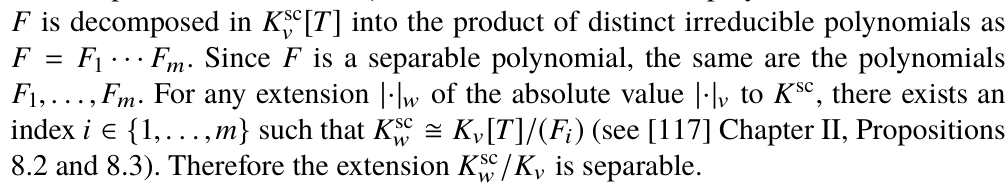
\includegraphics[width=\linewidth]{evidence/t6-original.png}
\end{center}
\noindent{\small Original PDF205 / printed189; crop rectangle $(50,491,386,553)$ in PDF coordinates.}

The extra $\mathrm{sc}$ in the factorization ring is real and should be removed.
But the quotient's left side \emph{already reads} $K_w^{\rm sc}$, and the following “Therefore” sentence also correctly uses $w$. The old second allegation is withdrawn; moving it to the next sentence would reproduce the same misreading. Inbox issue I-0007 records the blueprint's inaccurate quotation. The accepted blueprint and old report are preserved.

\subsection{E1--E3: qualifications rather than additional major errors}\label{e1}
\textbf{E1: cylinder reduction (PDF213--214 / printed197--198).}
The general-case paragraph on p.~214 treats a function “which can be written in the form” $g\circ\pi_{L_2/K_2}$. This naturally restricts attention to cylinder functions; p.~213 already invokes a monotone-class reduction. It does not establish that the authors falsely asserted finite-stage factorization for every measurable function. Add a sentence extending from cylinders by monotone classes or finite-measure uniqueness. This is a high-confidence expository clarification, not a confirmed false universal statement. Current \code{towerFibreMeasure_eq} and \code{fibreLIntegral_tower} perform the extension.

\textbf{E2: integrability in Proposition 3.4.10 (PDF211 / printed195).}
The surrounding discussion constructs an adelic extension; the proposition and displayed proof emphasize measurability of logarithmic evaluations. The other axiom, integrability for nonzero elements, follows immediately from finite descent, equation (3.19), and Proposition 3.4.9. Explicitly citing that step would close an exposition gap. No counterexample or theorem failure is claimed. Current \code{integrable_log_measure} and \code{algebraicExtension} supply it.

\textbf{E3: zero coefficients (PDF203 / printed187).}
After (3.11), the integrability sentence treats $\ln|\mu_i|_\omega$ for every coefficient. A minimal polynomial can have zero coefficients, for example $T^2-2$. Ordinary $\ln0$ is undefined, and the convention $\ln0=-\infty$ is not an integrable real function. Omit zero coefficients from the maximum (which already includes 0), or explicitly assign them value 0. The root bound and conclusion do not change. Because the audit did not exhaustively search all book-wide logarithm conventions, this is a \emph{medium-confidence notation qualification}, not a major source error. The blueprint explicitly omits zero terms; Lean's \code{integrable_coefficientLogBound} handles its totalized logarithm.


\clearpage
\section{Formalization corrections and boundaries}\label{formal}
\subsection{F1: integrability must be tested by a nonnegative integral}
\loc{210--211}{194--195}
After (3.18), the source defines signed fibre integration only when $I_{L/K}(|f|)$ is real-valued. Proposition 3.4.9 then treats integrable functions and $L^1$. Using a totalized real Bochner integral to test integrability of an infinite fibre can conceal divergence, because it returns 0 for a nonintegrable function. For measurable $f$, the correct test is
\[
 f\in L^1(\nu_L)\quad\Longleftrightarrow\quad
 \int_{\Omega_K}^{+}\!\int_{M_{L,\omega}}^{+}|f(x)|\,d\PP_{L,\omega}(x)\,d\nu_K(\omega)<\infty.
\]
The extended nonnegative integral retains divergence information. Current
\code{Algebraic.integrable_measure_iff}, signed disintegration, and the $L^1$ operator follow this distinction.
F1 is a \textbf{historical formalization-interface correction}, not a manuscript defect; confidence is high.

\subsection{F2: no unconditional pointwise signed tower identity}
\loc{210--214}{194--198}
An earlier formalization statement quantified over arbitrary real functions without measurability or integrability assumptions. That exceeds the source's integration domains. The baseline preserves the curve equivalence and projection compatibility, with the integral consequences formulated as
\begin{align*}
 I^+_{L_1/K}(I^+_{L_2/L_1}f)&=I^+_{L_2/K}f
 &&\text{for nonnegative measurable }f,\text{ pointwise},\\
 I_{L_1/K}(I_{L_2/L_1}f)&=I_{L_2/K}f
 &&\text{for integrable real }f,\ \nu_K\text{-a.e.}
\end{align*}
The second identity accommodates arbitrary a.e.\ representatives; nonintegrable fibres can lie over a null set. Totalization is not an unconditional Fubini theorem. F2 is another \textbf{correction of an overstrong historical Lean statement}, not an original-text error; confidence is high. The audit verifies the present interfaces and the mathematical distinction. The historical SHA \code{25eb9cd} cited by the old records is absent from this ledger, so the original revision was not independently replayed.

\subsection{F3: the number-field example uses a different disclosed normalization}
\loc{186--187}{170--171}
Section 3.2.2 extends the normalized finite absolute values $|p|_p=p^{-1}$ and assigns mass $n_{\mathfrak p}=[K_{\mathfrak p}:\Q_p]$.
The baseline \code{Examples/NumberFields.lean} instead uses Mathlib's
$N(\mathfrak p)^{-\operatorname{ord}_{\mathfrak p}}$ and finite-place mass 1, together with a zero-mass trivial place. The module and blueprint state those formulas, but these are \textbf{not literally the same source curve data}.

A reproducible witness is $K=\Q(\sqrt2)$ and $\mathfrak p=(\sqrt2)$.
Here $\mathcal O_K=\Z[\sqrt2]$, $\mathcal O_K/\mathfrak p=\mathbf F_2$,
$(2)=\mathfrak p^2$, and the local degree is 2. Thus
\[
 (|2|_{\mathfrak p},\nu\{\mathfrak p\})_{\rm source}=(1/2,2),\qquad
 (|2|_{\mathfrak p},\nu\{\mathfrak p\})_{\rm Lean}=(1/4,1).
\]
Generally, the latter absolute value is the $n_{\mathfrak p}$th power of the former, so weighted logarithms and the corresponding heights agree. Both constructions support a product formula; the proved properness result is not contradicted. Equality of weighted logarithms does not imply separate equality of absolute values and measures, or an absolute-value-preserving identity morphism.

F3 is a \textbf{disclosed alternative model requiring an explicit comparison with the source normalization}, with high confidence. Inbox issue I-0008 records the boundary; accepted code was not repaired in this read-only task.

\subsection{Other matters that must not be counted as source errors}
Proposition 3.6.2 uses a normal closure in the manuscript; current Lean uses positive fibre weights and measurable images of projections to prove orbit-maximum measurability. Both routes are valid, including inseparable extensions. Every real function on a finite fibre is integrable, so F1's infinite-fibre problem cannot be transplanted here. Pullback of absolute values is naturally a right action under the usual composition convention; this does not invalidate the measurability result. The use of finite embedding comparisons for conjugate heights in \S3.5 is also an ordinary valid proof-route change.

Zero elements and zero vectors require care when comparing source domains with totalized Lean definitions; the chosen totalization alone is not a manuscript error. The three audited imported-Mathlib graph warnings (I-0004) and missing legacy page transcriptions (I-0001) are project metadata limitations. They are not errors in the original PDF. The audit used that PDF directly where transcriptions were missing.

\section{What changes relative to the older report}
The eight-page report dated 16 September 2026,
\code{docs/chen-moriwaki-formalization-review.tex/pdf}, is preserved. The present report independently revisits its claims rather than translating or concatenating them.

\begin{longtable}{@{}p{19mm}p{\dimexpr\linewidth-19mm-2\tabcolsep\relax}@{}}
\toprule Old ID & Present disposition\\\midrule\endhead
S1 & Retain the divisibility counterexample and verify all relevant hypotheses. The later minimal-polynomial conclusion is a consequence of the false degree setup, not a second counterexample under the asserted equality.\\[4pt]
S2 & Strengthen the evidence from a general inverse-limit warning to an actual adelic counterexample. Acknowledge that compact cylinders and Carathéodory extension are already used in the source.\\[4pt]
T1--T5 & Confirm local notation/domain corrections.\\[4pt]
T6 & Retain only the factorization-ring correction. Withdraw the alleged quotient subscript error; the next sentence is also correct.\\[4pt]
T7--T11 & Confirm, recording both domain slips in T7. Correcting T10--T11 still leaves S1 unresolved in the printed proof.\\[4pt]
T12 & Retain the direction of correction, but correct the old quotation: the source has $\E_{L_2/L}$, not $\E_{L_2/L_1}$.\\[4pt]
E1 & Downgrade to an optional explanatory addition; the surrounding monotone-class context does not support an accusation of false universal factorization.\\[4pt]
F1--F2 & Retain as historical formalization corrections, strictly outside the manuscript-error count.\\[4pt]
New scope & Add S3, T13--T20, E2--E3, and F3. Recent \code{source-corrections.md} entries already pointed to S3 and T13; this audit rechecks them and adds examples, precise locators, and calibrated classifications.\\\bottomrule
\end{longtable}

The repair directions in the baseline \code{source-corrections.md} broadly agree with S1--S3, but do not replace source inspection. Its treatment of S2 should not suggest that the source lacked the compactness/Carathéodory route. T6 shows why agreement between an old report and its blueprint quotation is not independent evidence of a source typo.

The final report is in English pursuant to the user's later Horizon conversation I-0010. The superseded Chinese draft was preserved as a session attempt before replacement; it is not a second final report.

\clearpage
\appendix
\section{Exact Lean and blueprint attachments}
All paths are relative to the project root and all lines refer to the pinned revision.
In the table, Lean paths omit \code{ArakelovGeometry/AdelicCurve/}, except paths beginning \code{ExternalResults/}, which omit only \code{ArakelovGeometry/}. Names omit \code{ArakelovGeometry.AdelicStructure.} unless explicitly marked as full.
Blueprint paths omit \code{blueprint/src/}. These conventions determine exact full names and paths; \code{findings.json} writes them without abbreviation.

Attachments identify the relevant existing object, corrected interface, or repair consumer. They do not certify the report's new counterexamples in Lean. Navigational prose has no fabricated theorem attachment.

\small
\begin{longtable}{@{}p{11mm}p{\dimexpr\linewidth-11mm-2\tabcolsep\relax}@{}}
\toprule ID & Exact declaration / label and file location\\\midrule\endhead
S1 & Full name: \code{IntermediateField.exists_finite_descent}\newline \code{ExternalResults/AlgebraicTowerSupport.lean:242}\par\smallskip \code{Algebraic.fibreLIntegral_tower_projFinite}\newline \code{Extension/Algebraic/TowerCylinder.lean:54}\par\smallskip \code{Algebraic.towerFibreMeasure_eq}\newline \code{Extension/Algebraic/Tower.lean:25}\par\smallskip BP \code{lem:finite-descent-separable}\newline \code{algebraic.tex:1178}\par\smallskip BP \code{lem:descended-base-change}\newline \code{algebraic.tex:1270}\par\smallskip BP \code{rem:algebraic-tower-source-repair}\newline \code{algebraic.tex:1309}\par\smallskip BP \code{lem:algebraic-tower-cylinders}\newline \code{algebraic.tex:1444}\\[6pt]
S2 & \code{Algebraic.fibreMeasurableSpace}\newline \code{Extension/Algebraic/Basic.lean:365}\par\smallskip \code{Algebraic.fibreMeasurableSpace_eq_generateFrom}\newline \code{Extension/Algebraic/CylinderContent.lean:173}\par\smallskip \code{Algebraic.fibreCylinderAddContent_isSigmaSubadditive}\newline \code{Extension/Algebraic/CylinderContent.lean:280}\par\smallskip \code{Algebraic.fibreProbabilityMeasure}\newline \code{Extension/Algebraic/Probability.lean:30}\par\smallskip BP \code{def:projective-measurable}\newline \code{algebraic.tex:145}\par\smallskip BP \code{rem:cylinder-borel-distinction}\newline \code{algebraic.tex:298}\par\smallskip BP \code{lem:cylinder-premeasure}\newline \code{algebraic.tex:437}\par\smallskip BP \code{def:algebraic-fibre-probability}\newline \code{algebraic.tex:509}\\[6pt]
S3 & \code{integrable_κ}\newline \code{Basic.lean:119}\par\smallskip \code{heightArchimedeanConstant}\newline \code{Height/Polynomial.lean:144}\par\smallskip \code{polynomialHeight_mul_le}\newline \code{Height/Polynomial.lean:239}\par\smallskip \code{ofReal_polynomialHeight_mul_le_measure_Ωinf}\newline \code{Height/Polynomial.lean:331}\par\smallskip \code{heightArchimedeanConstant_algebraicExtension}\newline \code{Height/Extension.lean:60}\par\smallskip \code{affineHeight_minpoly_coeff_le}\newline \code{Height/MinimalPolynomial.lean:109}\par\smallskip \code{finite_affineHeight_le_degree_le}\newline \code{Height/Northcott.lean:65}\par\smallskip \code{finite_absoluteHeight_le_degree_le}\newline \code{Height/ProjectiveNorthcott.lean:65}\par\smallskip BP \code{def:height-archimedean-constant}\newline \code{northcott.tex:148}\par\smallskip BP \code{rem:northcott-archimedean-error}\newline \code{northcott.tex:297}\par\smallskip BP \code{thm:northcott}\newline \code{northcott.tex:574}\\[6pt]
T1 & \code{ParameterSpaceExtension.tsum_fibreWeight}\newline \code{Extension/Separable/FibreIntegral.lean:36}\par\smallskip BP \code{lem:fibre-normalization}\newline \code{separable.tex:29}\\[6pt]
T2 & \code{ParameterSpaceExtension.fibreIntegral_log_eq_log_norm}\newline \code{Extension/Separable/Construction.lean:31}\par\smallskip BP \code{lem:fibre-log-norm}\newline \code{separable.tex:1012}\\[6pt]
T3 & \code{log_apply_le_rootBound}\newline \code{Extension/RootBounds.lean:75}\par\smallskip BP \code{lem:log-root-bound}\newline \code{separable.tex:1113}\\[6pt]
T4 & \code{log_apply_le_rootBound}\newline \code{Extension/RootBounds.lean:75}\par\smallskip BP \code{lem:log-root-bound}\newline \code{separable.tex:1113}\\[6pt]
T5 & \code{ParameterSpaceFinExtension}\newline \code{Extension/Finite/Construction.lean:34}\par\smallskip BP \code{def:finite-parameters}\newline \code{finite.tex:152}\\[6pt]
T6 & \code{ParameterSpaceFinExtension.fieldRange_completion_separableClosure}\newline \code{Extension/Finite/Construction.lean:275}\par\smallskip BP \code{lem:completion-separable-closure}\newline \code{finite.tex:274}\par\smallskip BP \code{rem:completion-factorization-indices}\newline \code{finite.tex:316}\\[6pt]
T7 & \code{ParameterSpaceFinExtension.towerMeasurableEquiv}\newline \code{Extension/Finite/Tower.lean:192}\par\smallskip BP \code{lem:finite-tower-parameters}\newline \code{finite.tex:618}\par\smallskip BP \code{rem:finite-tower-evaluation-domain}\newline \code{finite.tex:776}\\[6pt]
T8 & \code{Algebraic.DescendsToFiniteFiber}\newline \code{Extension/Algebraic/CylinderContent.lean:66}\par\smallskip BP \code{def:algebraic-cylinders}\newline \code{algebraic.tex:309}\\[6pt]
T9 & \code{Algebraic.measurable_fibreLIntegral}\newline \code{Extension/Algebraic/Measure.lean:202}\par\smallskip BP \code{prop:algebraic-kernel-measurable}\newline \code{algebraic.tex:712}\\[6pt]
T10 & \code{ParameterSpaceExtension.fibreProbabilityMeasure_singleton}\newline \code{Extension/Finite/Probability.lean:42}\par\smallskip BP \code{lem:finite-fibre-sum}\newline \code{finite.tex:358}\\[6pt]
T11 & \code{ParameterSpaceFinExtension.lintegral_baseChangeFiber}\newline \code{Extension/Finite/BaseChange.lean:153}\par\smallskip BP \code{lem:descended-base-change}\newline \code{algebraic.tex:1270}\\[6pt]
T12 & \code{Algebraic.towerMeasurableEquiv}\newline \code{Extension/Algebraic/TowerBasic.lean:68}\par\smallskip BP \code{lem:algebraic-tower-spaces}\newline \code{algebraic.tex:1346}\\[6pt]
T13 & Full name: \code{ArakelovGeometry.AdelicCurve.RationalFunction.HorizontalPlace}\newline \code{Examples/RationalFunction/FinitePlaces.lean:31}\par\smallskip Full name: \code{ArakelovGeometry.AdelicCurve.RationalFunction.horizontalAbv}\newline \code{Examples/RationalFunction/FinitePlaces.lean:91}\par\smallskip Full name: \code{ArakelovGeometry.AdelicCurve.RationalFunction.morphismToRationals}\newline \code{Morphism/RationalFunction.lean:24}\par\smallskip BP \code{def:rational-horizontal-place}\newline \code{rational-finite-places.tex:9}\par\smallskip BP \code{ex:adelic-morphism-rational-function}\newline \code{rational-morphism.tex:200}\\[6pt]
T14 & Full name: \code{ArakelovGeometry.AdelicCurve.RationalFunction.integrable_log_polynomial_circle}\newline \code{Examples/RationalFunction/Archimedean.lean:108}\par\smallskip BP \code{lem:rational-polynomial-circle-log-integrable}\newline \code{rational-morphism.tex:65}\\[6pt]
T15 & Full name: \code{ArakelovGeometry.AdelicCurve.RationalFunction.archimedeanDomain}\newline \code{Examples/RationalFunction/Archimedean.lean:36}\par\smallskip Full name: \code{ArakelovGeometry.AdelicCurve.RationalFunction.ArchimedeanPlace}\newline \code{Examples/RationalFunction/Archimedean.lean:40}\par\smallskip BP \code{def:rational-circle-parameters}\newline \code{rational-morphism.tex:4}\\[6pt]
T16 & Full name: \code{ArakelovGeometry.AdelicCurve.Hom.comp}\newline \code{Morphism/Basic.lean:111}\par\smallskip BP \code{lem:adelic-morphism-comp}\newline \code{morphisms.tex:90}\\[6pt]
T17 & Full name: \code{ArakelovGeometry.AdelicCurve.RationalFunction.augmentedRationalAdelicCurve}\newline \code{Examples/RationalFunction/Construction.lean:63}\par\smallskip Full name: \code{ArakelovGeometry.AdelicCurve.RationalFunction.augmentedRationalAdelicStructure_horizontal}\newline \code{Examples/RationalFunction/Construction.lean:79}\par\smallskip BP \code{def:augmented-rational-adelic-curve}\newline \code{rational-morphism.tex:171}\\[6pt]
T18 & No direct Lean declaration: navigational prose.\\[6pt]
T19 & \code{ParameterSpaceExtension.fibreIntegral_comp_restrict}\newline \code{Extension/Separable/FibreIntegral.lean:161}\par\smallskip BP \code{prop:fibre-restriction}\newline \code{separable.tex:144}\\[6pt]
T20 & \code{ParameterSpaceExtension.fibreIntegral_comp_proj}\newline \code{Extension/Separable/FibreIntegral.lean:150}\par\smallskip BP \code{cor:fibre-pullback}\newline \code{separable.tex:131}\\[6pt]
E1 & \code{Algebraic.fibreLIntegral_tower_projFinite}\newline \code{Extension/Algebraic/TowerCylinder.lean:54}\par\smallskip \code{Algebraic.towerFibreMeasure_eq}\newline \code{Extension/Algebraic/Tower.lean:25}\par\smallskip BP \code{lem:algebraic-tower-cylinders}\newline \code{algebraic.tex:1444}\par\smallskip BP \code{thm:algebraic-tower-lintegral}\newline \code{algebraic.tex:1573}\\[6pt]
E2 & \code{Algebraic.integrable_log_measure}\newline \code{Extension/Algebraic/Construction.lean:26}\par\smallskip \code{algebraicExtension}\newline \code{Extension/Algebraic/Construction.lean:42}\par\smallskip BP \code{prop:algebraic-log-integrable}\newline \code{algebraic.tex:1087}\par\smallskip BP \code{def:algebraic-extension}\newline \code{algebraic.tex:1102}\\[6pt]
E3 & \code{integrable_coefficientLogBound}\newline \code{Extension/RootBounds.lean:42}\par\smallskip BP \code{lem:coefficient-log-envelope}\newline \code{separable.tex:1094}\\[6pt]
F1 & \code{Algebraic.integrable_measure_iff}\newline \code{Extension/Algebraic/Integral.lean:29}\par\smallskip BP \code{prop:algebraic-integrability}\newline \code{algebraic.tex:770}\\[6pt]
F2 & Full name: \code{ArakelovGeometry.exists_equiv_algebraicExtension_algebraicExtension}\newline \code{Extension/Algebraic/Tower.lean:167}\par\smallskip \code{Algebraic.fibreIntegral_tower}\newline \code{Extension/Algebraic/Tower.lean:132}\par\smallskip BP \code{thm:algebraic-tower}\newline \code{algebraic.tex:1667}\par\smallskip BP \code{rem:signed-tower-domain}\newline \code{algebraic.tex:1712}\\[6pt]
F3 & \code{placeRep}\newline \code{Examples/NumberFields.lean:105}\par\smallskip \code{placeWeight}\newline \code{Examples/NumberFields.lean:113}\par\smallskip \code{placeRep_mk_finitePlace}\newline \code{Examples/NumberFields.lean:160}\par\smallskip \code{placeWeight_mk_finitePlace}\newline \code{Examples/NumberFields.lean:169}\par\smallskip \code{numberFieldAdelicStructure}\newline \code{Examples/NumberFields.lean:218}\par\smallskip BP \code{def:number-field-place-data}\newline \code{number-fields.tex:362}\par\smallskip BP \code{def:number-field-adelic-structure}\newline \code{number-fields.tex:434}\\[6pt]
\bottomrule
\end{longtable}
\normalsize

\section{Coverage and limitations}
All 41 entries in \code{docs/source-result-index.json} for \S\S3.3--3.7 were checked against blueprint attachments, source-facing statements, and issue-relevant proof bodies. This does not mean independently re-proving all 1,413 constants in the declaration inventory or auditing every imported Mathlib proof.

\begin{longtable}{@{}p{25mm}p{36mm}p{\dimexpr\linewidth-61mm-4\tabcolsep\relax}@{}}
\toprule Section & Original PDF / printed pages & Actual coverage\\\midrule\endhead
3.3 & 194--204 / 178--188 &
12 index entries: setup, 3.3.1--3.3.6, and 3.3.7(1)--(5). Finite separable parameters, fibre weights, measurability, measure construction, logarithmic norm, and integrability. All old notation candidates and the surrounding proofs were visually checked.\\[4pt]
3.4 & 204--215 / 188--199 &
14 entries: setup and 3.4.1--3.4.13. Finite general extensions, inverse-limit fibres, probability, integrability, properness, tower compatibility, and restriction. Fresh scrutiny of S1/S2 and all T5--T12/E1/F1--F2.\\[4pt]
3.5 & 215--218 / 199--202 &
8 entries: 3.5.1--3.5.7 plus polynomial-height setup. Height extension, Northcott, conjugates, product bound, coefficient bound, and finite-extension corollary; original proof and current finite-$\kappa$ route compared.\\[4pt]
3.6 & 218--219 / 202--203 &
2 entries: 3.6.1--3.6.2. Invariant measurability and maximum over a finite orbit, including the normal-closure and inseparability context.\\[4pt]
3.7 & 219--220 / 203--204 &
5 entries: definition, composition, and three examples. Morphism domains, kernels/integrals, extension/restriction examples, and the rational-function morphism.\\[4pt]
3.2.5 & 188--190 / 172--174 &
Original rational-function construction, horizontal points, Mahler weights, circle parameters, product-formula discussion, and comparison with Example 3.7.2(3).\\\bottomrule
\end{longtable}

\noindent\textbf{Additional original-page checks.}
Page 1: version cover.
PDF57 / printed41: local polynomial product estimate.
PDF78 / printed62: the actual Corollary 1.2.33, to check T20.
PDF184--185 / printed168--169: the full \S3.1 definitions and three propositions.
PDF186--187 / printed170--171: \S\S3.2.1--3.2.3.
PDF193 / printed177: \S\S3.2.7--3.2.9.
The union of visually checked original pages is
\[
 \{1,57,78\}\ \cup\ \{184,\ldots,190\}\ \cup\ \{193,\ldots,220\}.
\]
Section 3.2.4 was visible on adjacent pages but was not an independent audit target; \S3.2.6 and Chapter 6 were outside the mathematical scope.

Earlier code was also sampled for basic definitions, integrability of $\kappa$, trivial curves, restriction, amalgamation, number fields, and the principal rational-function constructions and product formulas. The object in \code{Examples/FunctionFields.lean} is $k(T)/\PP^1_k$, not an arbitrary regular projective curve from \S3.2.1; the blueprint discloses this restriction. The current \S3.2.5 morphism formalization does not claim its separate product formula. These boundaries preclude saying that every item of Chapter 3 has been formalized.

\noindent\textbf{Historical records.}
Inputs included the old report, \code{source-corrections.md}, \code{proof-status.md}, the declaration inventory, blueprint coverage, and recent height, automorphism, and morphism commits/review records.
Commit \code{77d5464} records the finite-exponent error term,
\code{3148ff0} projective Northcott, and \code{f589e8a} and \code{fe4feea} the \S\S3.6 and 3.7 checks.
Historical build and axiom-audit results are contextual evidence, not fresh runs in this audit.

\noindent\textbf{Limits.}
No later manuscript edition or author errata were compared. This is not an exhaustive audit of all 466 pages, nor a claim that the inspected pages have no other errors.
The counterexamples and arguments in S1--S3 are independently reviewed mathematical evidence, not new Lean theorems.
No broad rebuild or Lean probe was run. Global strict source coverage remains limited by missing legacy transcriptions for PDF194--214, and the three known imported-Mathlib graph warnings remain metadata boundaries.

\section{Reproduction and delivery checks}
\code{provenance.json} pins the manuscript, older report, and principal inputs by hash.
\code{findings.json} gives the 29 findings with exact source and formalization locators, qualifications, and the 41-entry coverage list.
\code{evidence/crops.json} specifies the original-page crop used for T6.
Raw independent review records and the separate S2 adjudication are retained under \code{evidence/}; the final English catalogue and this report contain the adjudicated conclusions.

Compile with XeLaTeX and the installed TeX Gyre Pagella / DejaVu Sans Mono fonts:
\begin{quote}\texttt{bash build.sh}\end{quote}
The script runs three passes, rejects missing-glyph, unresolved-reference, and overfull-box diagnostics, keeps auxiliaries in a temporary directory, and updates only \code{report.pdf} in the report directory.
The final factual/locator review, honesty review, and per-page rendering inspection are recorded in \code{review-checks.json}. These checks certify the delivered report's reviewed scope and layout; they do not certify the manuscript as error-free.
All deliverables are committed in the Horizon ledger, with accepted project sources and old reports preserved.

\end{document}
